\documentclass{article}
\usepackage[UKenglish]{babel}
\usepackage[UKenglish]{isodate}
\usepackage[utf8]{inputenc}
\usepackage{fullpage}

\usepackage{mathtools}
\usepackage{amsthm}
\usepackage{mathrsfs}
\usepackage{amsfonts}

\usepackage[linesnumbered,ruled,vlined]{algorithm2e}
\usepackage{tikz}
\usepackage[capitalize]{cleveref}

\usetikzlibrary{arrows,fit,positioning,trees,cd}

\crefname{algocf}{algorithm}{Algorithms}
\Crefname{algocf}{Algorithm}{Algorithms}

\theoremstyle{definition}
\newtheorem{definition}{Definition}
\newtheorem{example}{Example}

\newcommand\pfun{\mathrel{\ooalign{\hfil$\mapstochar\mkern5mu$\hfil\cr$\to$\cr}}}

\DeclareMathOperator{\dom}{dom}
\DeclareMathOperator{\Imm}{Im}
\DeclareMathOperator{\Doms}{Doms}
\DeclareMathOperator{\Vars}{Vars}
\DeclareMathOperator{\WMC}{WMC}

\title{Empowering Domain Recursion in Symmetric Weighted First-Order Model Counting}

\begin{document}
\maketitle

\section{Basic Definitions}

\paragraph{Things I might need to explain.}
\begin{itemize}
\item notation: $\Imm$
\item atom, literal, constant, predicate, variable
\item inequality constraint
\item $\Vars$, $\Vars(c) = \Vars(P) \cup \Vars(N) \cup \Vars(C)$
\item $\Doms$ on both formulas and clauses. $\Doms(c) = \Imm \delta_c$, and $\Doms(\phi) = \bigcup_{c \in \phi} \Doms(c)$.
\item substitution
\item size of a domain, how each domain is partitioned into two during compilation.
\item maybe: notation for partial function, notation for powerset, domain size
\item notation for projection (or avoid it?)
\item $\WMC$
\item constraint removal operation
\item two parts: compilation and inference.
\item introduce and use arrows for bijections, injections, set inclusions, etc.
\item $\emptyset$ for an empty partial map.
\end{itemize}

Let $\mathscr{V}$ be the set of circuit nodes.

\paragraph{TODO}
\begin{itemize}
\item later: maybe mathcal instead of mathscr
\item maybe $\pi$ is global enough to have a more unique name
\item maybe $c[\beta, \gamma]$ is better than $c \ast (\beta, \gamma)$
\end{itemize}

\begin{definition}
  A \emph{domain} is a set with elements not used anywhere else.\footnote{In the context of functions, the domain of a function $f$ retains its usual meaning and is denoted $\dom(f)$.} Let $\mathscr{D}$ be the set of all domains and $\mathscr{C} \subset \mathscr{D}$ be the subset of domains introduced as a consequence of constraint removal. Note that both sets (can) expand during the compilation phase.

Let $\pi\colon \mathscr{D} \pfun \mathscr{D}$ be a partial endomorphism on $\mathscr{D}$ that denotes the \emph{parent} relation, i.e., if $\pi(d) = e$ for some $d, e \in \mathscr{D}$, then we call $e$ the parent (domain) of $d$, and $e$ a child of $d$. Intuitively, $\pi$ arranges all domains into a forest---thus, we often use graph theoretical terminology to describe properties of and relationships between domains.
\end{definition}

\begin{definition}
  A \emph{clause} is a triple $c = (P, N, C, \delta_c)$, where $P$ and $N$ are sets of atoms interpreted as positive and negative literals respectively, $C$ is a set of inequality constraints, and $\delta_c\colon \Vars(c) \to \mathscr{D}$ is a function that maps all variables in $c$ to their domains. Two clauses $c$ and $d = (P', N', C', \delta_d)$ are \emph{isomorphic} (written $c \cong d$) if there is a bijection $\beta\colon \Vars(c) \to \Vars(d)$ such that $c\beta = d\beta$. TODO: we will always use this subscript notation for the $\delta$'s. Equality of clauses is defined in the usual way (i.e., all variables, domains, etc. must match).
\end{definition}

A \emph{formula} is a set of clauses.

We use hash codes to efficiently check whether a recursive relationship between two formulas is plausible. (It is plausible if the formulas are equal up to variables and domains.) The hash code of a clause $c = (P, N, C, \delta_c)$ combines the hash codes of the sets of constants and predicates in $c$, the numbers of positive and negative literals (i.e., $|P|$ and $|N|$), the number of inequality constraints $|C|$, and the number of variables $|\Vars(c)|$. The hash code of a formula $\phi$ combines the hash codes of all its clauses and is denoted $\#\phi$.

\section{Identifying Possibilities for Recursion}

\begin{definition}[Notation]
  For any clause $c = (P, N, C, \delta_c)$, bijection $\beta\colon \Vars(c) \to V$ (for some set of variables $V$) and function $\gamma\colon \Doms(c) \to \mathscr{D}$, let $c \ast (\beta, \gamma) = d$ be the clause with all occurrences of any variable $v \in \Vars(c)$ in $P$, $N$, and $C$ replaced with $\beta(v)$ (so $\Vars(d) = V$) and $\delta_d\colon V \to \mathscr{D}$ defined as $\delta_d \coloneqq \gamma \circ \delta_c \circ \beta^{-1}$. In other words, $\delta_d$ is the unique function that makes the following diagram commute:
  \[
  \begin{tikzcd}
    \Vars(c) \ar[r, tail, two heads, "\beta"] \arrow[d, swap, "\delta_c"] & V = \Vars(d) \ar[d, dashed, "\exists!\delta_d"] \\
    \Doms(c) \ar[r, swap, "\gamma"] & \mathscr{D}.
  \end{tikzcd}
  \]
\end{definition}

\begin{algorithm}[t]
  \caption{A recursive function for checking whether one can reuse the circuit for computing $\WMC(\phi)$ to compute $\WMC(\psi)$. Both $\phi$ and $\psi$ are formulas, and $\rho\colon \Doms(\phi) \protect\pfun \Doms(\psi)$ is a partial map.}
  \label{alg:recursion}
  \SetKwProg{Fn}{Function}{:}{}
  \SetKw{KwRet}{yield}
  \SetKwFunction{identifyRecursion}{identifyRecursion}
  \SetKwFunction{findHistory}{traceAncestors}
  \SetKwFunction{generateMaps}{generateMaps}
  \SetKwFunction{constructDomainMap}{constructDomainMap}
  \SetKwData{suitable}{suitableBijection}
  \SetKwData{found}{foundConstraintRemoval}
  \Fn{\identifyRecursion{$\phi$, $\psi$, $\rho = \emptyset$, $\found = {\normalfont \texttt{false}}$}}{
    \lIf{$|\phi| \ne |\psi|$ {\bf or} $\#\phi \ne \#\psi$}{\Return{\normalfont \texttt{null}}}
    \If{$\phi = \emptyset$}{
      \lIf{$\found$}{\Return{$\rho$}}
      \Return{\normalfont \texttt{null}}\;
    }
    \ForEach{clause $c \in \phi$\label{line:for1}}{
      \ForEach{clause $d \in \psi$ such that $\#d = \#c$\label{line:for2}} {
        \ForEach{$(\beta, \gamma) \in \generateMaps{$c$, $d$, $\rho$}$ such that $c \ast (\beta, \gamma) = d$\label{line:generateMaps}}{
          $\found' \gets \found$\;
          $\suitable \gets \texttt{true}$\;
          \ForEach{$e \in \Doms(c)$\label{line:vars}}{
            $\found'' \gets \findHistory{$e$, $\gamma(e)$}$\;
            \If{$\found'' = {\normalfont \texttt{null}}$}{
              $\suitable \gets \texttt{false}$\;
              break\;
            }
            \lIf{$\found''$}{$\found' \gets \texttt{true}$}
          }
          \If{\suitable}{
            $\rho'' \gets \identifyRecursion{$\phi \setminus \{\, c \,\}$, $\psi \setminus \{\, d \,\}$, $\rho \cup \gamma$, $\found'$}$\;\label{line:recursion}
            \lIf{$\rho'' \ne {\normalfont \texttt{null}}$}{\Return{$\rho''$}}
          }
        }
      }
      \Return{\normalfont \texttt{null}}\;
    }
  }
  \Fn{\generateMaps{$c$, $d$, $\rho$}}{
    \ForEach{bijection $\beta\colon \Vars(c) \to \Vars(d)$\label{line:bijection}}{
      $\gamma \gets \constructDomainMap{$\Vars(c)$, $\delta_c$, $\delta_d$, $\beta$, $\rho$}$\;
      \lIf{$\gamma \ne {\normalfont \texttt{null}}$}{\KwRet{$(\beta, \gamma)$}}
    }
  }
  \Fn{\constructDomainMap{$V$, $\delta_c$, $\delta_d$, $\beta$, $\rho$}}{
    $\gamma \gets \emptyset$\;
    \ForEach{$v \in V$}{
      \lIf{$\delta_c(v) \in \dom(\rho)$ {\bf and} $\rho(\delta_c(v)) \ne \delta_d(\beta(v))$}{\Return{\normalfont \texttt{null}}}
      \lIf{$\delta_c(v) \not\in \dom(\gamma)$}{$\gamma \gets \gamma \cup \{\, \delta_c(v) \mapsto \delta_d(\beta(v)) \,\}$}
      \lElseIf{$\gamma(\delta_c(v)) \ne \delta_d(\beta(v))$}{\Return{\normalfont \texttt{null}}}
    }
    \Return{$\gamma$}\;
  }
  \Fn{\findHistory{$d$, $e$}}{
    $\found \gets \texttt{false}$\;
    \While{$e \ne d$ {\bf and} $e \in {\normalfont \dom}(\pi)$}{
      \lIf{$e \in \mathscr{C}$}{$\found \gets \texttt{true}$}
      $e \gets \pi(e)$\;
    }
    \lIf{$e = d$}{\Return{\found}}
    \Return{\normalfont \texttt{null}}\;
  }
\end{algorithm}

\begin{figure}[t]
  \centering
  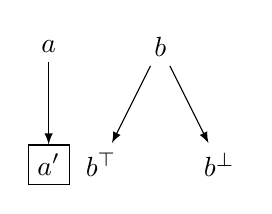
\begin{tikzpicture}[edge from parent/.style={draw,-latex}]
    %% \node[draw,circle,fill=violet!10] (circuit) {} child {
    %%   node[draw,circle,fill=violet!10] (bmaker) {$\diamondsuit$}
    %%   child {node[draw,circle,fill=violet!10] {}
    %%     child {node[draw,circle,fill=violet!10] {}}
    %%     child {node[draw,circle,fill=violet!10] {}
    %%       child {node[draw,circle,fill=violet!10] {}}
    %%       child {node[draw,circle,fill=violet!10] {}
    %%         child {node[draw,circle,fill=violet!10] {}}
    %%         child {node[draw,circle,fill=violet!10] (amaker) {$\heartsuit$}
    %%           child {node[draw,circle,fill=violet!10] (ref) {}
    %%             child {node[draw,circle,fill=violet!10] {}}
    %%           }
    %%         }
    %%       }
    %%     }
    %%   }
    %% };
    \node (a) {$a$} child {node[draw,rectangle] (aprime) {$a'$}};
    \node[right=1 cm of a] (b) {$b$}
    child {node (btop) {$b^\top$}}
    child {node (bbot) {$b^\bot$}};
    %% \node[draw,fit=(a) (aprime) (b) (btop) (bbot)] {};
    %% \draw[-latex] (ref) edge[densely dotted,bend left=90] (circuit);
    %% \draw[-latex,color=teal] (aprime) edge[densely dashed] node[xshift=2mm,color=teal] {$0$} (amaker);
    %% \draw[-latex,color=teal] (btop) edge[bend left=50,densely dashed] node[xshift=6mm,color=teal] {$0$} (bmaker);
    %% \draw[-latex,color=teal] (bbot) edge[bend left=50,densely dashed] node[yshift=-2mm,color=teal] {$1$} (bmaker);
  \end{tikzpicture}
  \caption{The forest of domains from \cref{example}. The directed edges correspond to the pairs of domains in $\pi$ but in the opposite direction, e.g., $\pi(a') = a$. The domain enclosed in a rectangle is the only domain created by constraint removal, i.e., $\mathscr{C} = \{\, a' \,\}$.}
  \label{fig:example}
\end{figure}

The function \texttt{traceAncestors} returns \texttt{null} if domain $d \in \mathscr{D}$ is not an ancestor of domain $e \in \mathscr{D}$. Otherwise, it returns \texttt{true} if the size of $e$ is guaranteed to be strictly smaller than the size of $d$ (i.e., there is domain created by the constraint removal rule on the path from $d$ to $e$) and \texttt{false} if their sizes will be equal at some point during inference.

Notation: For partial functions $\alpha, \beta\colon A \pfun B$ such that $\alpha|_{\dom(\alpha) \cap \dom(\beta)} = \beta|_{\dom(\alpha) \cap \dom(\beta)}$, we write $\alpha \cup \beta$ for the unique partial function such that $\alpha \cup \beta|_{\dom(\alpha)} = \alpha$, and $\alpha \cup \beta|_{\dom(\beta)} = \beta$.

\paragraph{TODO}
\begin{itemize}
\item explain why $\rho \cup \gamma$ is possible
\item explain what the second return statement is about and why a third one is not necessary
\item mention which one is the main function, what each function takes and returns
\item explain the yield keyword
\item in the example below: write down both formula using the Forclift format
\end{itemize}

The algorithm could be improved in two ways:
\begin{itemize}
\item by constructing a domain map first and then using it to reduce the number of viable variable bijections.
\item by similarly using the domain map $\rho$.
\end{itemize}
However, it is not clear that this would result in an overall performance improvement, since the number of variables in instances of interest never exceeds three and the identity bijection is typically the right one.

Diagramatically, \texttt{constructDomainMap} attempts to find $\gamma\colon \Doms(c) \to \Doms(d)$ such that the following diagram commutes (and returns \texttt{null} if such a function does not exist):
\[
\begin{tikzcd}
  \Vars(c) \ar[r, tail, two heads, "\beta"] \arrow[d, swap, "\delta_c"] & \Vars(d) \ar[d, "\delta_d"] \\
  \Doms(c) \ar[r, dashed, "\gamma"] \ar[d, hookrightarrow] & \Doms(d) \ar[d, hookrightarrow] \\
  \mathscr{D} \ar[r, swap, "\rho"] & \mathscr{D}.
\end{tikzcd}
\]

\begin{example} \label{example}
  Let $\phi$ be the formula
  \begin{align}
    \forall X \in a. \forall Y \in b. \forall Z \in b. Y \ne Z &\implies \neg p(X, Y) \lor \neg p(X, Z)\label{phi1} \\
    \forall X \in a. \forall Y \in b. \forall Z \in a. X \ne Z &\implies \neg p(X, Y) \lor \neg p(Z, Y).\label{phi2}
  \end{align}
  and $\psi$ be the formula
  \begin{align}
    \forall X \in a'. \forall Y \in b^\bot. \forall Z \in b^\bot. Z \ne Y &\implies \neg p(X, Y) \lor \neg p(X, Z)\label{psi1} \\
    \forall X \in a'. \forall Y \in b^\bot. \forall Z \in a'. X \ne Z &\implies \neg p(X, Y) \lor \neg p(Z, Y)\label{psi2}
  \end{align}

  The relevant domains and the definition of $\pi$ is in \cref{fig:example}. Since $\#\phi = \#\psi$, and the formulas are non-empty, the algorithm proceeds with the for-loops on \cref{line:for1,line:for2,line:generateMaps}. Suppose $c$ in the algorithm refers to \cref{phi1}, and $d$ to \cref{psi1}. Since both clauses have three variables, in the worst case, function \texttt{generateMaps} would have $3!=6$ bijections to check. Suppose the identity bijection is picked first. Then \texttt{constructDomainMap} is called with the following parameters:
  \begin{itemize}
  \item $V = \{\, X, Y, Z \,\}$,
  \item $\delta_c = \{\, X \mapsto a, Y \mapsto b, Z \mapsto b \,\}$,
  \item $\delta_d = \{\, X \mapsto a', Y \mapsto b^\bot, Z \mapsto b^\bot \,\}$,
  \item $\beta = \{\, X \mapsto X, Y \mapsto Y, Z \mapsto Z \,\}$,
  \item $\rho = \emptyset$.
  \end{itemize}
  Since $\delta_i(Y) = \delta_i(Z)$ for $i \in \{\, c, d \,\}$, \texttt{constructDomainMap} returns $\gamma = \{\, a \mapsto a', b \mapsto b^\bot \,\}$. Thus, \texttt{generateMaps} yields its first pair of maps $(\beta, \gamma)$ to \cref{line:generateMaps}. Furthermore, the pair satisfies the $c \ast (\beta, \gamma) = d$ condition.

  Since $\pi(a') = a$, and $a' \in \mathscr{C}$, \texttt{traceAncestors($a$, $a'$)} returns \texttt{true}, which sets $\textsf{foundConstraintRemoval}'$ to \texttt{true} as well. When $e = b$, however, \texttt{traceAncestors}($b$, $b^\bot$) returns \texttt{false} since $b^\bot$ is a descendant of $b$ but not created by the constraint removal compilation rule. On \cref{line:recursion}, a recursive call to \texttt{identifyRecursion($\phi'$, $\psi'$, $\gamma$, true)} is made, where $\phi'$ and $\psi'$ are new formulas with one clause each: \cref{phi2} and \cref{psi2}, respectively.

  Again we have two non-empty formulas with equal hash codes, so \texttt{generateMaps} is called with $c$ set to \cref{phi2}, $d$ set to \cref{psi2}, and $\rho = \{\, a \mapsto a', b \mapsto b^\bot \,\}$. Suppose \cref{line:bijection} picks the identity bijection first again. Then \texttt{constructDomainMap} is called with the following parameters:
  \begin{itemize}
  \item $V = \{\, X, Y, Z \,\}$,
  \item $\delta_c = \{\, X \mapsto a, Y \mapsto b, Z \mapsto a \,\}$,
  \item $\delta_d = \{\, X \mapsto a', Y \mapsto b^\bot, Z \mapsto a' \,\}$,
  \item $\beta = \{\, X \mapsto X, Y \mapsto Y, Z \mapsto Z \,\}$,
  \item $\rho = \{\, a \mapsto a', b \mapsto b^\bot \,\}$.
  \end{itemize}
  Since $\beta$ and $\rho$ `commute' (TODO: as in the diagram above), and there are no new domains in $\Doms(c)$ and $\Doms(d)$, $\gamma$ exists and is equal to $\rho$. Again, the returned pair $(\beta, \gamma)$ satisfies the condition $c \ast (\beta, \gamma) = d$. This $\gamma$ passes the \texttt{traceAncestors} checks exactly the same way as the one before, and \cref{line:recursion} calls \texttt{identifyRecursion($\emptyset$, $\emptyset$, $\rho$, true)}, which immediately returns $\rho = \{\, a \mapsto a', b \mapsto b^\bot \,\}$ as the final answer. This means that one can indeed use a circuit for $\WMC(\phi)$ to compute $\WMC(\psi)$ by replacing every mention of $a$ with $a'$ and every mention of $b$ with $b^\bot$.
\end{example}

\subsection{Evaluation}

This $\rho$ is saved as a parameter of the new circuit node. During inference, there is a domain size map $\sigma\colon \mathscr{D} \to \mathbb{N}_0$, which gets updated to
\[
\sigma'(x) =
\begin{cases}
  \sigma(\rho(x)) & \text{if } x \in \dom(\rho) \\
  \sigma(x) & \text{otherwise}
\end{cases}
\]
for all $x \in \mathscr{D}$.

\section{New Operations}

TODO: compilation rules, node types, their evaluation during inference.

\subsection{Improved Domain Recursion}

The original version of domain recursion is here \cite{DBLP:conf/nips/Broeck11}.

\subsection{Constraint Removal}

\section{Other Topics}

\begin{itemize}
\item domains, smoothing, and avoiding infinite cycles
\item new rules that don't create nodes (e.g., duplicate removal, unconditional contradiction detection, etc.)
\end{itemize}

\section{Circuit Evaluation}

TODO: new node types, their algebraic/graphical representation, what info they hold, and how they're created.

TODO: describe evaluation of: and, counting, constraint removal, ref, unit, contradiction, improved domain recursion. Most of this will be from \cite{DBLP:conf/ijcai/BroeckTMDR11}.

\bibliographystyle{acm}
\bibliography{notes}

\end{document}
